\documentclass[10pt,oneside,a4paper]{article}

\usepackage[]{babel}
\usepackage[IL2]{fontenc}
\usepackage[utf8]{inputenc}
\usepackage{graphicx}
\usepackage{url}
\usepackage{hyperref}
\usepackage{cite}

\pagestyle{headings}

\title{Challenges in Semantic Search: Understanding User Intent and Context\thanks{Semester Project in Methods of Engineering Work, Academic Year 2022/23}}

\author{Aliaksei Zimnitski \\[2pt]
{\small \texttt{xzimnitski@stuba.sk}}\\
Coauthor: MSc. Mirwais Ahmadzai \\[2pt]
{\small \texttt{mirwais.ahmadzai@stuba.sk}}\\
{\small Slovenská technická univerzita v Bratislave}\\
{\small Fakulta informatiky a informačných technológií}\\
}

\date{\small \today}

\begin{document}

\maketitle

\begin{abstract}
Semantic search is a vital technology in the field of information retrieval. It plays a pivotal role in enhancing search accuracy by focusing on understanding user intent and context. This article delves into the multifaceted challenges faced by semantic search systems, offering insights into the intricacies of ambiguity resolution and the need to adapt to dynamic language. It underscores the importance of leveraging natural language processing and artificial intelligence to address these challenges effectively. By comprehending these complexities, we can unlock the full potential of semantic search in information retrieval.
\end{abstract}

\section{Introduction}
Semantic search has revolutionized information retrieval, offering the promise of more accurate and context-aware search results. However, it is not without its challenges. This paper delves into the intricacies of semantic search and the hurdles it encounters when trying to understand user intent and context.

The advent of semantic search has brought about a paradigm shift in the way we seek and access information. Unlike traditional keyword-based searches, semantic search aims to understand the meaning behind the queries, making it a cornerstone of modern information retrieval. It goes beyond surface-level keyword matching and focuses on deciphering the intricacies of human language, emphasizing user intent and context \cite{BaezaYates1999} \cite{Manning2008}.

\section{Resolving User Intent Ambiguity}
One of the primary challenges in semantic search is the ambiguity of user intentions. Consider a simple query like "Apple." It could refer to the technology company, the fruit, or even a record label. Semantic search engines must decipher the relevant context to provide accurate results.

To tackle this issue, semantic search systems employ a variety of techniques, including natural language processing, entity recognition, and context analysis. These methods help disambiguate user queries and retrieve relevant results. However, the challenge persists, as language is nuanced and context-dependent.

User intent ambiguity is further compounded by the evolution of language and the emergence of new terms and concepts. For instance, words like "tweet" or "cloud" have taken on entirely new meanings in the digital age. Semantic search systems must adapt to these changes to remain effective \cite{Smith2018}.

\section{Leveraging Knowledge Graphs}
Semantic search systems benefit greatly from knowledge graphs that provide structured information about a wide range of topics. Google's Knowledge Graph is a notable example, offering a vast reservoir of interconnected entities and their relationships. By tapping into this knowledge graph, semantic search engines can enhance their understanding of user queries and context. This allows them to provide more relevant and context-aware results \cite{Singhal2012}.

Additionally, there's Wikidata, a collaborative project that compiles structured data about diverse subjects. Wikidata serves as a valuable resource for semantic search engines, enabling them to access extensive information and cross-references across various domains. This, in turn, helps in disambiguating terms and enriching search results \cite{Vrandecic2014}.


\begin{figure}[h]
\centering
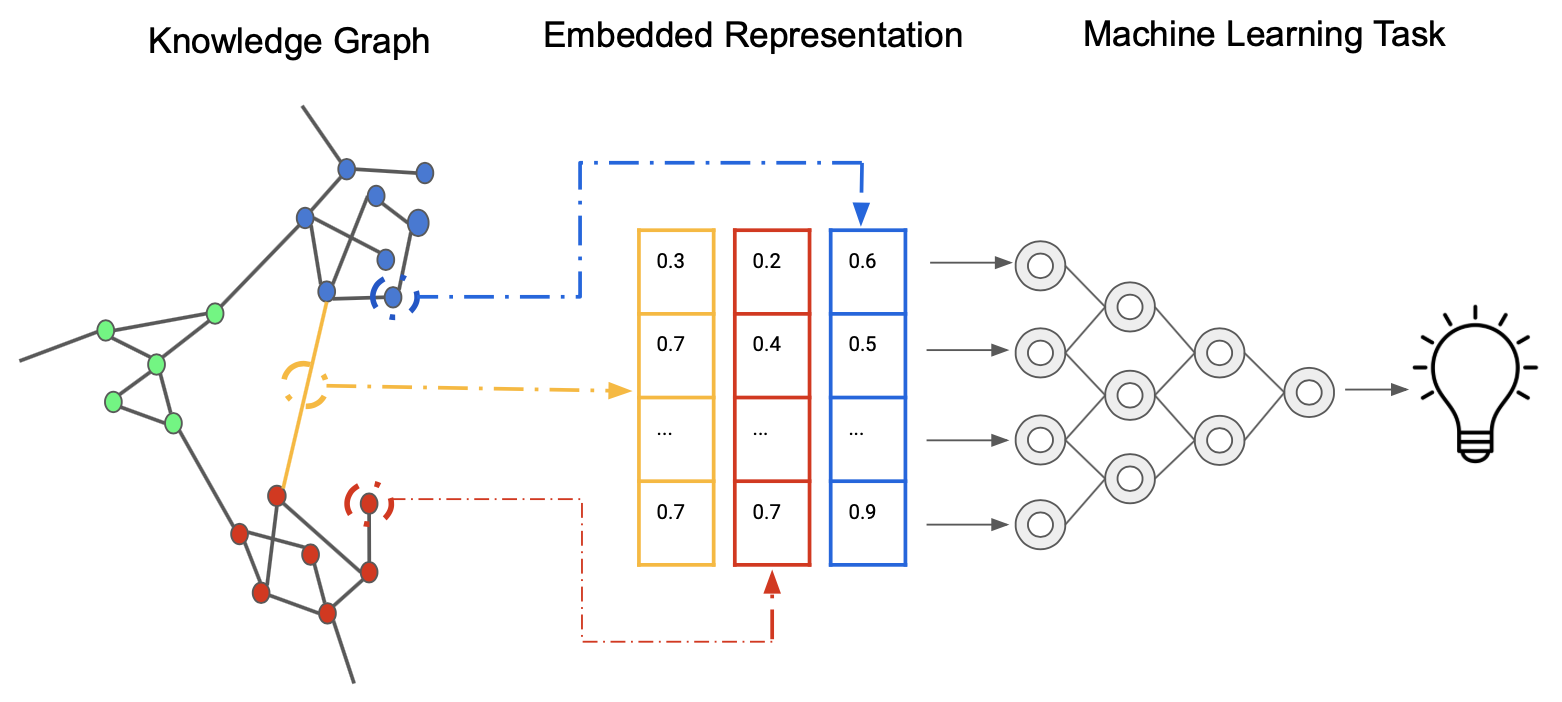
\includegraphics[scale=0.4]{LKG.png}\
\end{figure}

\section{Adapting to Dynamic Language and Context}
Another significant challenge in semantic search is adapting to the dynamic nature of language and evolving context. Language is a living entity, and the meanings of words can shift over time. The same word may have different connotations or refer to distinct entities in various contexts.

For instance, consider the word "jaguar." Depending on the context in which it is used, it can refer to a luxury car, a large feline animal, or even a sports team. Semantic search engines must navigate these complexities to ensure users receive the most relevant search results.

Adapting to dynamic language and context requires constant updates and refinements. Semantic search systems need to learn and evolve alongside language, incorporating new terms and understanding shifting meanings. This necessitates the integration of artificial intelligence and machine learning to keep pace with linguistic developments \cite{Wilson2019}.


\section{NLP in Semantic Search}
Natural Language Processing (NLP) is the driving force behind the capabilities of semantic search. NLP techniques enable semantic search systems to understand and interpret the complexities of human language. They facilitate entity recognition, sentiment analysis, and context understanding, all of which contribute to providing more accurate search results.

One notable aspect of NLP is sentiment analysis, which enables semantic search engines to gauge the sentiment or emotional tone of text. For instance, a search for "best smartphone" may yield different results based on whether the user is looking for positive or negative reviews. NLP plays a crucial role in determining this sentiment and tailoring search results accordingly \cite{Jurafsky2020}.

\begin{figure}[h]
\centering
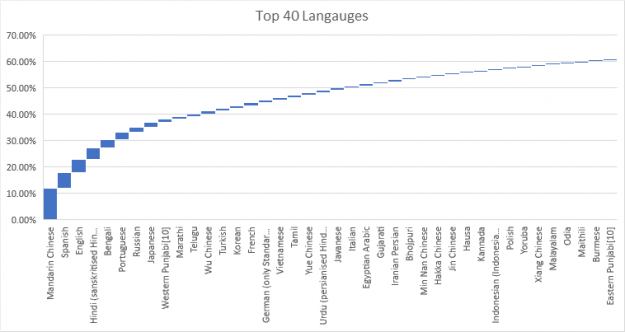
\includegraphics[scale=0.6]{NLP.png}\
\caption{List of Top 40 languages by total number of native speakers}
\end{figure}

\section{Future Developments}
The future of semantic search holds the promise of further transforming how we access information. Continued advancements in natural language processing, machine learning, and knowledge graphs will contribute to more sophisticated and accurate search results. The evolution of semantic search will play a significant role in shaping the future of information retrieval \cite{Jurafsky2020}.

\section{Challenges in User Privacy and Data Security}
With the growing capabilities of semantic search and the increasing amount of user data being processed, challenges related to user privacy and data security have come to the forefront. Semantic search systems require access to a vast amount of user data to understand intent and context effectively. However, this raises concerns about how this data is collected, stored, and used.

In recent years, there have been instances of data breaches and privacy violations involving prominent technology companies. These incidents underscore the need for robust data security measures in semantic search systems. As technology evolves, ensuring user privacy and data protection will be an ongoing challenge that requires attention and innovation.

\section{Scalability and Efficiency}
As the usage of semantic search continues to grow, ensuring scalability and efficiency becomes a significant challenge. Large-scale semantic search systems must handle a vast number of user queries and process extensive amounts of data. Ensuring that these systems can provide real-time responses while maintaining efficiency is a complex task.

Researchers and developers are actively exploring solutions to enhance the scalability of semantic search systems, including distributed computing techniques and optimization algorithms. These efforts are crucial to meet the demands of an ever-expanding user base.

\section{Conclusion}
In conclusion, while semantic search offers tremendous potential for improving search accuracy and user experience, it faces substantial challenges related to understanding user intent and context. The ambiguity of user intentions, adapting to dynamic language, and emerging challenges in user privacy and data security are significant hurdles.

Semantic search technology will continue to evolve, offering more refined and context-aware results. As language and context complexities persist, addressing these challenges is crucial for unlocking the full capabilities of semantic search and providing users with the information they seek in an increasingly digital world.

Semantic search plays a pivotal role in enhancing search accuracy by focusing on understanding user intent and context. The challenges it faces, including user intent ambiguity and adapting to dynamic language, underscore the need for continuous innovation and research in the field. By addressing these challenges effectively, we can unlock the full potential of semantic search in information retrieval and provide users with more accurate and context-aware search results.

\newpage
\nocite{*}
\bibliographystyle{plain}
\bibliography{article}

\end{document}
